\documentclass[a4paper]{article}

\usepackage[a4paper,top=2cm,bottom=2cm,left=0.5cm,right=0.5cm,marginparwidth=1.75cm]{geometry}
\usepackage[utf8]{inputenc}
\usepackage[english, russian]{babel}
\usepackage[]{amsmath,amsfonts,amssymb,amsthm,mathtools}
\usepackage[]{wasysym}
\usepackage[]{float}
\usepackage{multicol}
\usepackage{amsfonts}
\usepackage{indentfirst}
\usepackage{longtable}
\usepackage{natbib}
\usepackage{mathrsfs}
\usepackage{wrapfig}
\usepackage{graphicx}
\usepackage{mathtext}
\usepackage{amsmath}
\usepackage{siunitx} % Required for alignment
\usepackage{subfigure}
\usepackage{multirow}
\usepackage{rotating}
\usepackage[T1,T2A]{fontenc}
\usepackage{caption}
\usepackage{gensymb}


\date{\today}
\title{Лабораторная работа 3.2.6}
\author{Сидорчук Максим}

\begin{document}
\maketitle

\section{Цель работы}
Изучение работы высокочувствительного зеркального гальванометра магнитоэлектрической системы в режимах измерения постоянного тока и электрического заряда.

\section{В работе используются:}
Зеркальный гальванометр с осветителем и шкалой, источник постоянного напряжения, делитель напряжения, магазин сопротивлений, эталонный конденсатор, вольтметр, переключатель, ключи, линейка

\section{Теоретические положения}

\textit{Баллистический гальванометр} -- электроизмерительный прибор магнитоэлектрической системы, отличающийся высокой чувствительностью к току и сравнительно большим периодом свободных колебаний. \par
На помещённую в магнитное поле обтекаемую током рамку гальванометра действуют момент закрученной нити, момент магнитных сил и тормозящий момент (зависит от сил сопротивления воздуха и от вихревых токов). Учитывая все эти моменты, уравнение движения рамки принимает вид
\begin{center}
    $\ddot \varphi + 2 \gamma \dot \varphi + \omega_0^2\varphi = KI $,
\end{center}
где $\gamma$ -- коэффициент затухания подвижной системы гальванометра, $\omega_0$ -- собственная частота колебаний рамки

Динамическая постоянная гальванометра определяется при пропускании через рамку постоянного тока:
\begin{center}
    $C_I = \frac{I}{\varphi} = \frac{D}{BSN}$,
\end{center}
где $B$ - индукция магнитного поля в рамке, $S$ - площадь одного витка рамки, $D$ - модуль кручения нити. \par
При пропускании коротких импульсов тока через баллистический гальванометр начальная скорость движения рамки пропорциональна электрическому заряду, прошедшему через рамку за всё время импульса. Отношение баллистических постоянных в критическом и свободном режимах равно $e$.

\section{Экспериментальная установка}
\subsection{Определение динамической постоянной}
\begin{figure}[H]
    \centering
    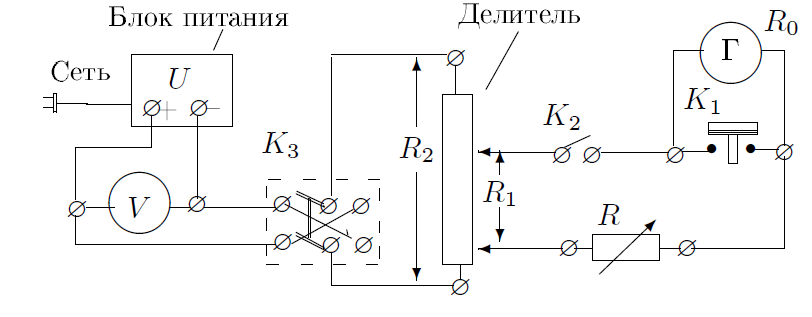
\includegraphics[width=10cm]{fig2.PNG}
    \caption{Схема установки для работы гальванометра в стационарном режиме}
    \label{fig:vac}
\end{figure}
% Постоянное напряжение $U = 1,5$В снимается с блока питания и измеряется вольтметром $V$. Ключ $K_3$ позволяет менять величину тока через гальванометр Г, делитель напряжения - менять величину тока в широких пределах. Ключ $K_2$ служит для включения гальванометра, кнопка $K_1$ -- для его успокоения. Магазин сопротивлений $R$ позволяет менять режим работы гальванометра от колебательного до апериодического. \par
% При малых $R_1$ сила тока, протекающего через гальванометр, может быть вычислена по формуле
Динамическую постоянную вычислим по формуле
\begin{equation}
    C_I = \frac{2aI}{x},
\end{equation}
где $a$ - расстояние от шкалы до зеркальца и $I$:
\begin{equation}
    I = U_0 \frac{R_1}{R_2} \frac{1}{R + R_0}.
\end{equation}

\subsection{Определение критического сопротивления гальванометра}
Выполняется с помощью той же цепи, что и на рис. 1.
% При больших $R$ движение рамки имеет колебательный характер, с уменьшением $R$ затухание увеличивается, и колебательный режим переходит в апериодический. \par
% Найдём логарифмический декремент затухания колебаний рамки  $\Theta$.
\begin{equation}
    \Theta = ln\frac{x_n}{x_{n+1}} = \gamma T = \frac{2\pi \gamma}{\sqrt{\omega_0^2 - \gamma^2}} = \frac{2\pi R_3}{\sqrt{(R_0 + R)^2 - R_3^2}}
\end{equation}

Рассчитаем критическое сопротивление по графику в координатах $X = (R_0^2 + R)$, $Y = 1/\Theta^2$
\begin{equation}
    R_\text{cr} = \frac{1}{2\pi}\sqrt{\frac{\triangle X}{\triangle Y}} - R_0
\end{equation}

\subsection{Определение баллистической постоянной и критического сопротивления гальванометра, работающего в баллистическом режиме}

Для изучения работы гальванометра в режиме измерения заряда используется схема, представленная на рис. 2.

\begin{figure}[H]
    \centering
    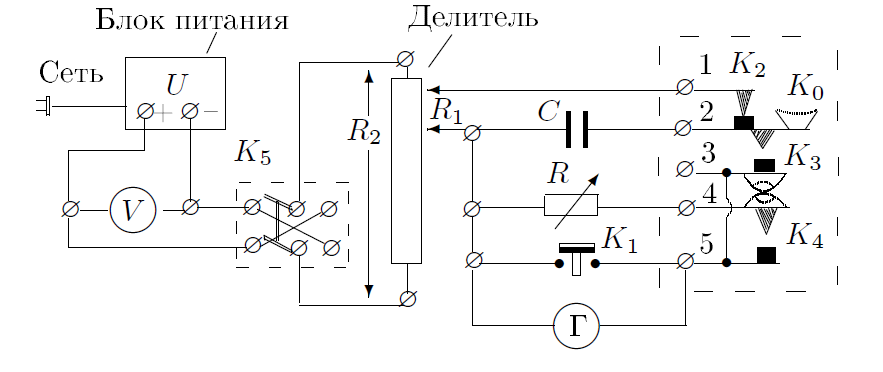
\includegraphics[width=10cm]{fig1.PNG}
    \caption{Схема установки для определения баллистической постоянной}
    \label{fig:vac}
\end{figure}

% При нормальном положении кнопки $K_0$ конденсатор $C$ заряжается до напряжения
% \begin{center}
%     $U_c = \frac{R_1}{R_2}U_0$
% \end{center}
% Заряд конденсатора равен
% \begin{center}
%     $q = \frac{R_1}{R_2}U_0 C$
% \end{center}
% При нажатии на ключ $K_0$ конденсатор отключается от источника постоянного напряжения и подключается к гальванометру. К моменту замыкания ключа $K_4$ весь заряд успевает пройти через гальванометр, рамка получает начальную скорость. 
Баллистическая постоянная гальванометра определяется при критическом сопротивлении
\begin{equation}
    C_\text{Qcr} = \frac{q}{\varphi_{max cr}} = 2a\frac{R_1}{R_2} \frac{U_0 C}{l_{max cr}}
\end{equation}

\section{Ход работы}
\begin{enumerate}
    \item Соберём схему согласно рис. 1. Снимем зависимость отклонения зайчика $x$ от сопротивления магазина $R$, увеличивая сопротивление магазина, но не меняя делителя. Результаты запишем в табл. 1. Ток в цепи рассчитаем по формуле (1) ($R_1/R_2 = 1/2000$, $U_0 = 1.47$ В, $R_0 = 280$ Ом.)

          \begin{table}[H]
              \centering
              \begin{center}
                  \caption{Зависимость отклонения зайчика от сопротивления, постоянный ток}
              \end{center}
              \vspace{0.1cm}
              \label{tab:my_label}
              \begin{tabular}{|c|c|c|c|c|c|c|c|c|c|}
                  \hline
                  $x$, мм  & 225  & 202  & 178  & 138  & 113  & 96   & 84   & 75   & 66   \\
                  \hline
                  $R$, кОм & 23   & 26   & 30   & 40   & 50   & 60   & 70   & 80   & 90   \\
                  \hline
                  $I$, нА  & 5.36 & 4.75 & 4.13 & 3.11 & 2.49 & 2.08 & 1.78 & 1.56 & 1.39 \\
                  \hline
              \end{tabular}
          \end{table}

          Графически представим результаты на графике $I = f(x)$ (рис. 3). Воcпользуемся методом наименьших квадратов для определения наклона прямой и погрешности его определения.

          \begin{figure}[h]
              \centering
              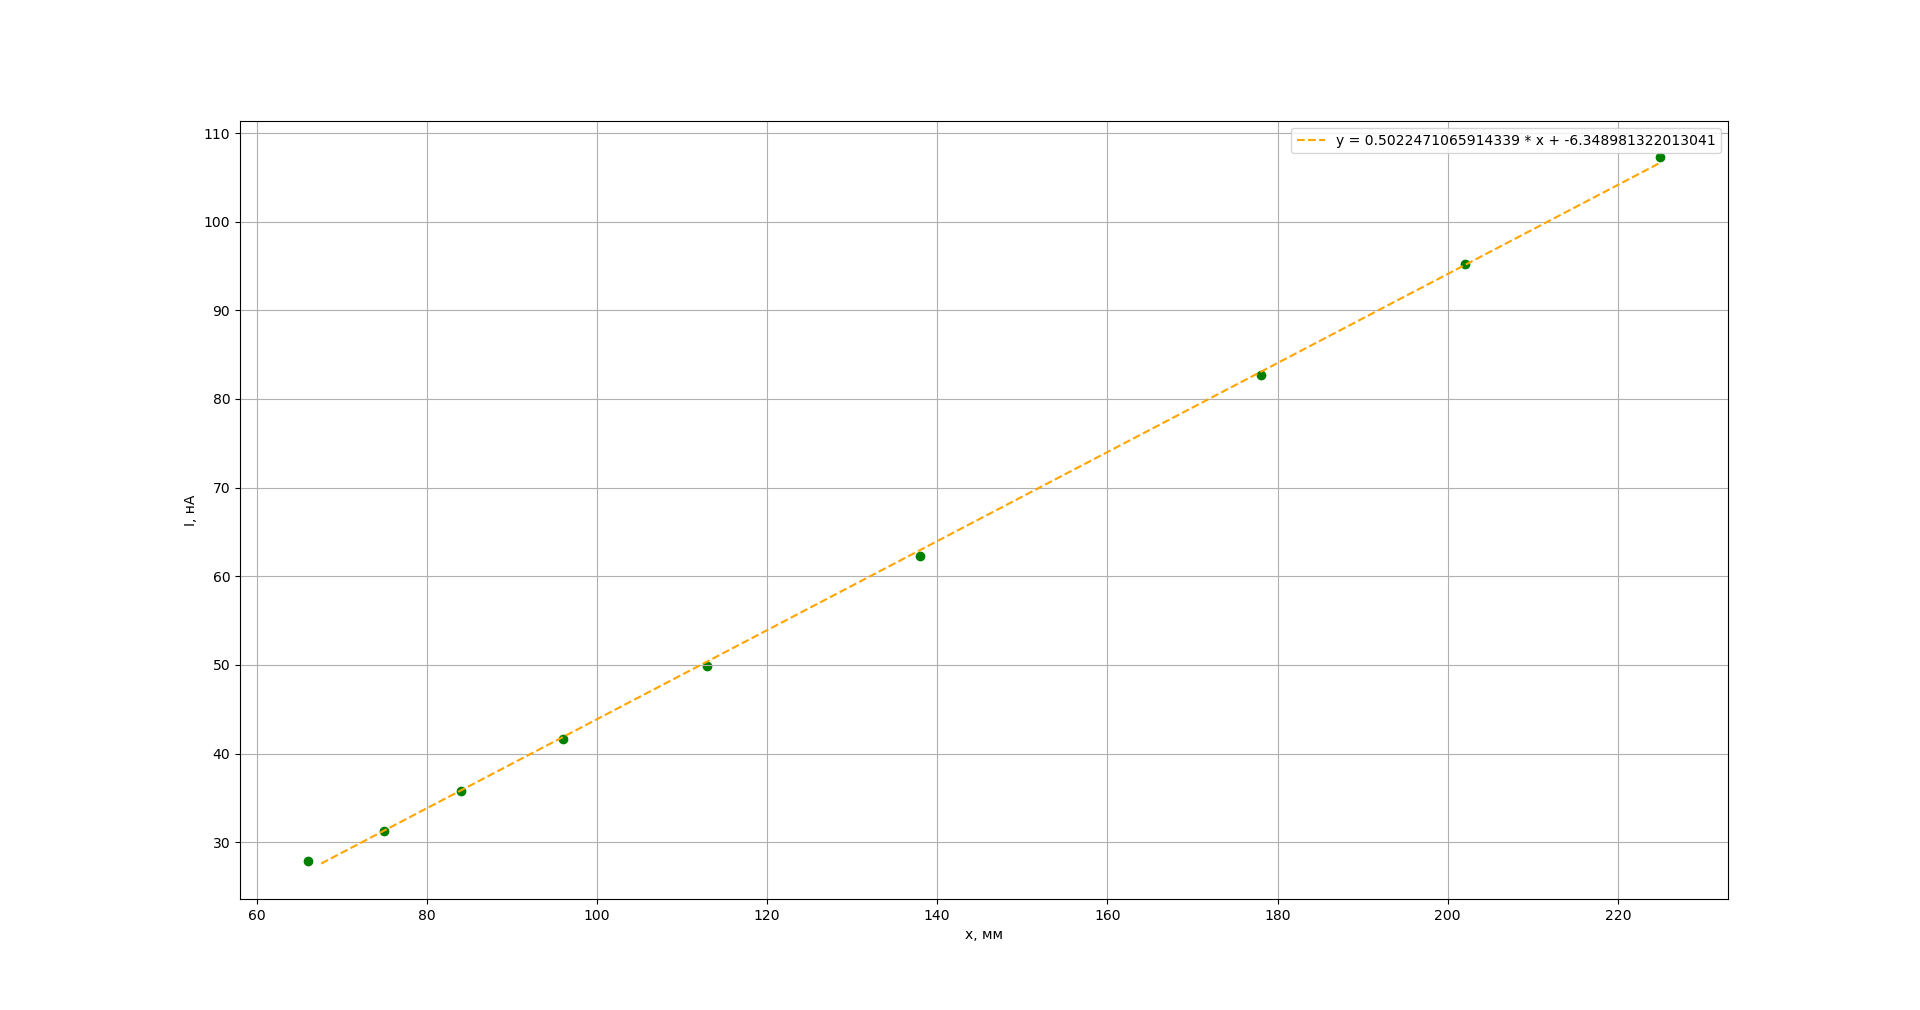
\includegraphics[width=\textwidth]{Figure_!.png}
              \caption{Определение динамической постоянной гальванометра}
              \label{fig:vac}
          \end{figure}

          \begin{center}
              $C_I = \frac{<xy>-<x><y>}{<x^2>-<x>^2} = 1.54$ нА/(мм/м)\\

              $\sigma_{\triangle C_I} = \frac{1}{\sqrt{n}} \sqrt{\frac{<y^2>-<y>^2}{<x^2>-<x>^2} - C_I^2} = 0.07$ нА/(мм/м)
          \end{center}

          Итого получаем
          \begin{center}
              $C_I = 1.54 \pm 0.07$ нА/(мм/м)
          \end{center}

    \item Рассчитаем логарифмический декремент затухания свободных колебаний рамки разомкнутого гальванометра. Результаты измерений занесём в табл. 2. Также определим приблизительно период свободных колебаний рамки.

          \begin{table}[H]
              \centering
              \begin{center}
                  \caption{Отклонения рамки при свободных колебаниях}
              \end{center}
              \vspace{0.1cm}
              \label{tab:my_label}
              \begin{tabular}{ |p{1.2cm}|p{1.2cm}|p{1.2cm}|p{1.2cm}|p{1.2cm}|p{1.2cm}|p{1.2cm}|p{1.2cm}|p{1.2cm}|p{1.2cm}|}
                  \hline
                  $x_1$, мм & $x_2$, мм & $x_3$, мм & $\Theta_1$ & $\Theta_2$ & $\Theta$ & $\sigma_\Theta$, мм & $T$, c \\
                  \hline
                  234       & 185 & 147   & 0.235     & 0.23       & 0.232      & 0.018    & 5.2                          \\
                  \hline
              \end{tabular}
          \end{table}

          Получили значение логарифмического декремента затухания свободных колебаний рамки
          \begin{center}
              $\Theta = 0.0641 \pm 0.0013$
          \end{center}

    \item При разомкнутом ключе $K_3$ определим наибольшее сопротивление магазина $R$, при котором при размыкании ключа зайчик не переходит за нулевое значение шкалы. Это сопротивление близко к критическому $R_\text{cr} \approx 7067$ Ом.

    \item Установим сопротивление магазина $R \approx 3R_\text{cr}$ и подберем делитель так, чтобы в стационарном режиме зайчик отклонялся на всю шкалу. Для расчёта $\Theta$ будем измерять два последовательных отклонения зайчика в одну сторону. Повторим измерения, увеличивая сопротивление магазина до $8R_\text{cr}$. Результаты занесём в табл. 3.

          \begin{table}[H]
              \centering
              \begin{center}
                  \caption{Зависимость отклонения зайчика от сопротивления, после размыкания ключа $K_3$}
              \end{center}
              \vspace{0.1cm}
              \label{tab:my_label}
              \begin{tabular}{ |c|c|c|c|c|c|c|c|c|c|c|c|c|c|c|c|c|c|}
                  \hline
                  $R$, кОм & 24.736 & 28.27 & 31.804 & 35.338 & 38.872 & 42.406 & 49.473 & 56.54 & 63.608 & 70.675 \\
                  \hline
                  $x1$, мм & 34     & 80    & 82     & 82     & 76     & 77     & 70     & 67    & 64     & 58     \\
                  \hline
                  $x2$, мм & 5      & 15    & 16     & 20     & 20     & 22     & 24     & 26    & 26     & 26     \\
                  \hline
                  $\Theta$ & 1.917  & 1.674 & 1.634  & 1.411  & 1.335  & 1.253  & 1.070  & 0.947 & 0.901  & 0.802  \\
                  \hline
              \end{tabular}
          \end{table}

          Построим график зависимости декремента затухания колебаний от сопротивления на магазине в координатах $1/\Theta^2 = f[(R+R_0)^2]$ (рис. 4). Используя формулу (4) и метод наименьших квадратов, определим по нему критическое сопротивление гальванометра. Также используя метода наименьших квадратов, оценим погрешность определения этой величины (формулы см. в п. 5.1)

          \begin{figure}[H]
              \centering
              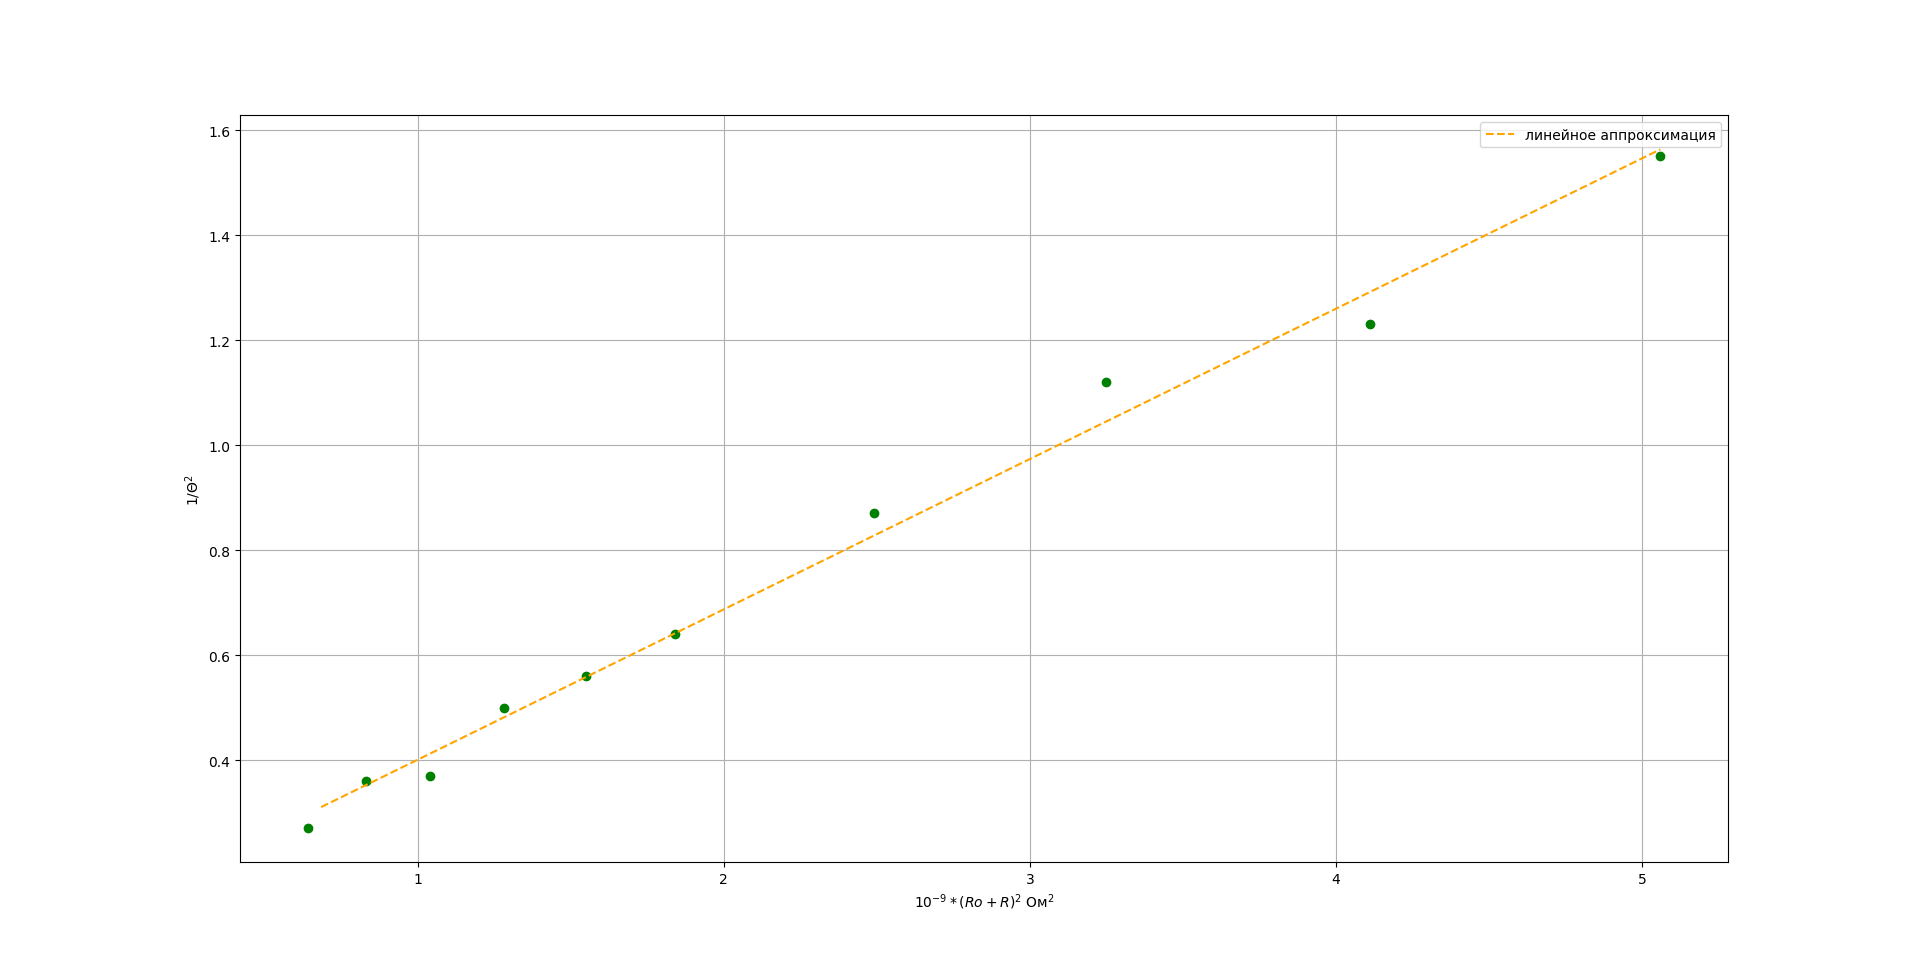
\includegraphics[width=\textwidth]{Figure_2.png}
              \caption{Определение критического сопротивления гальванометра, статический режим}
              \label{fig:vac}
          \end{figure}

          \begin{center}
              $R_\text{cr} = \frac{1}{2\pi}\sqrt{\frac{\triangle X}{\triangle Y}} - R_0$ \\
              $R_\text{cr} = 8929 \pm 140$ Ом
          \end{center}

    \item Перейдём к работе гальванометра в баллистическом режиме. Соберём схему по рис. 2. Разомкнём цепь $R$, отсоединив одну из клемм от магазина. Подберём делитель так, чтобы первый отбор соответствовал отклонению зайчика на всю школу. Для свободных колебаний $l_{max} = 237.8$ мм. \par
          Подключим магазин назад. Снимем зависимость величины первого отброса от $R$. Результаты занесём в табл. 4.


          \begin{table}[H]
              \centering
              \begin{center}
                  \caption{Зависимость отклонения зайчика от сопротивления, после размыкания ключа $K_3$}
              \end{center}
              \vspace{0.1cm}
              \label{tab:my_label}
              \begin{tabular}{ |c|c|c|c|c|c|c|c|c|c|c|c|c|c|c|c|c|c|c|}
                  \hline

                  $l_{max}$, мм & 22 & 21.3 & 21 & 20.8 & 20 & 19.1 & 17.8 & 16.1 & 14.4 & 11.3 & 5.5 & 10 & 8.7 & 8.1 & 6.8 & 6.1 \\
                  \hline
                  $R$, кОм      & 50 & 45.18 & 40.36 & 35.54 & 30.72 & 25.9 & 21.08 & 16.26 & 11.44 & 6.6 & 1.8 & 5.62 & 4.62 & 3.62 & 2.62 & 2.1 \\
                  \hline
              \end{tabular}
          \end{table}

          Построим график $l_\text{max} = f[(R_0 + R)^{-1}]$. По графику, используя метод наименьших квадратов, определим критическое сопротивление гальванометра ($l_\text{cr} = l_\text{max}/e$).
          \begin{figure}[H]
              \centering
              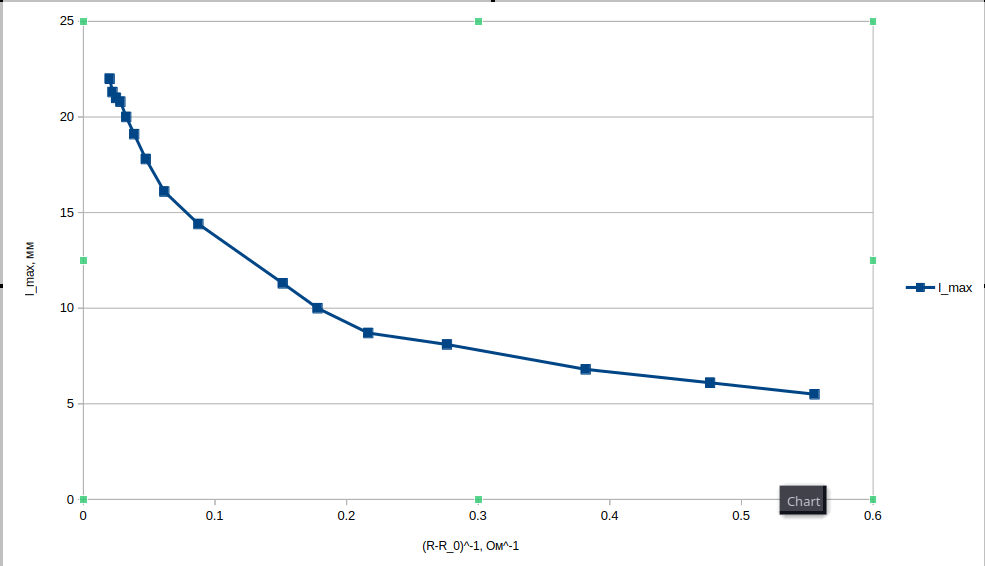
\includegraphics[width=\textwidth]{Figure_3.png}
              \caption{Определение критического сопротивления гальванометра, баллистический режим}
              \label{fig:vac}
          \end{figure}

          \begin{center}
              $a = 181, b = -111634$ \par
              $R_\text{cr} = (\frac{l_\text{cr} - a}{b})^-1 - R_0 = 7233 \pm 112$ Ом
          \end{center}

    \item По формуле (5) рассчитаем баллистическую постоянную в критическом режиме:
          \begin{center}
              $C_\text{Qcr} = \frac{q}{\varphi_\text{max cr}} = 2a\frac{R_1}{R_2} \frac{U_0 C}{l_\text{max cr}}$ \par

              $C_\text{Qcr} = (1.91 \pm 0.05) * 10^-9$ К/(мм/м)
          \end{center}

    \item Сравним время релаксации $t = R_0 C$ и период свободных колебаний гальванометра $T_0$
              $t = 0.00056 c \ll T = 5 c$
          Время релаксации много меньше периода свободных колебаний. Эксперимент корректен.

\end{enumerate}

\section{Вывод}

В ходе эксперимента был исследован принцип работы гальванометра в режиме постоянного тока и в баллистическом режиме. Определены динамическая и баллистическая постоянные гальванометра:

\begin{center}
    $C_I = 1.539 \pm 0.069$ нА/(мм/м) \hspace{1cm} $C_{Qcr}= 9.33 \pm 0.3 * 10^-9$ К/(мм/м)
\end{center}

Тремя разными способами было исследовано критическое сопротивление гальванометра. Результаты практически совпадают.

\begin{table}[h]
    \centering
    \begin{center}
        \caption{Значения $R_{cr}$, полученные разными способами}
    \end{center}
    \vspace{0.1cm}
    \label{tab:my_label}
    \begin{tabular}{ |p{4cm}|p{4cm}|p{4cm}|}
        \hline
        $R_{cr}$, Ом - подбор & $R_{cr}$, Ом  - по графику в стационарном режиме & $R_{cr}$, Ом - по графику в баллистическом режиме \\
        \hline
        $7067$                & $8929 \pm 140$                                    & $7233 \pm 112$                                      \\
        \hline
    \end{tabular}
\end{table}

\end{document}